% This file was created by tikzplotlib v0.9.1.
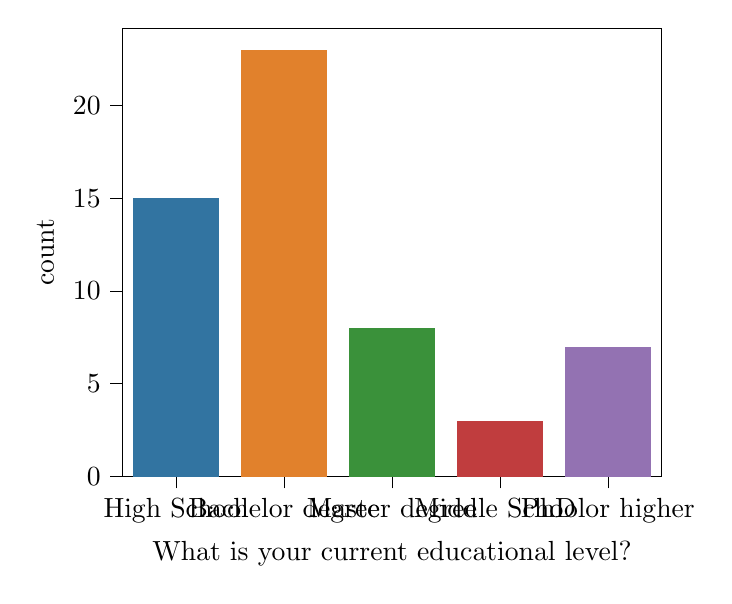
\begin{tikzpicture}

\definecolor{color0}{rgb}{0.194607843137255,0.453431372549019,0.632843137254902}
\definecolor{color1}{rgb}{0.881862745098039,0.505392156862745,0.173039215686275}
\definecolor{color2}{rgb}{0.229411764705882,0.570588235294118,0.229411764705882}
\definecolor{color3}{rgb}{0.75343137254902,0.238725490196078,0.241666666666667}
\definecolor{color4}{rgb}{0.578431372549019,0.446078431372549,0.699019607843137}

\begin{axis}[
tick align=outside,
tick pos=left,
x grid style={white!69.0196078431373!black},
xlabel={What is your current educational level?},
xmin=-0.5, xmax=4.5,
xtick style={color=black},
xtick={0,1,2,3,4},
xticklabels={High School,Bachelor degree,Master degree,Middle School,PhD or higher},
y grid style={white!69.0196078431373!black},
ylabel={count},
ymin=0, ymax=24.15,
ytick style={color=black}
]
\draw[draw=none,fill=color0] (axis cs:-0.4,0) rectangle (axis cs:0.4,15);
\draw[draw=none,fill=color1] (axis cs:0.6,0) rectangle (axis cs:1.4,23);
\draw[draw=none,fill=color2] (axis cs:1.6,0) rectangle (axis cs:2.4,8);
\draw[draw=none,fill=color3] (axis cs:2.6,0) rectangle (axis cs:3.4,3);
\draw[draw=none,fill=color4] (axis cs:3.6,0) rectangle (axis cs:4.4,7);
\end{axis}

\end{tikzpicture}
